\documentclass[11pt]{beamer}
%\usepackage{multicol}
\usepackage[vietnamese]{babel}
\usefonttheme[onlymath]{serif}
\usepackage{tgbonum}%chagne font

\usetheme[progressbar=frametitle]{metropolis}
\setbeamertemplate{frame numbering}[fraction]
\useoutertheme{metropolis}
\useinnertheme{metropolis}
\usefonttheme{metropolis}
\usecolortheme{spruce}
\setbeamercolor{background canvas}{bg=white}

\definecolor{mygreen}{rgb}{.125,.5,.25}
\usecolortheme[named=mygreen]{structure}

\usepackage{ragged2e}
\apptocmd{\frame}{}{\justifying}{}

\usepackage{graphicx,environ}
\usepackage{hyperref}

\NewEnviron{sourcefigure}[1][htbp]{%
	{\let\caption\relax\let\ref\relax
		\renewcommand{\label}[1]{%
			\gdef\sfname{sf:##1}}%
		\setbox1=\hbox{\BODY}}% Capture \label
	\global\expandafter\let\csname\sfname\endcsname\BODY% Capture entire figure
	\begin{figure}[#1]
		\BODY
	\end{figure}
}
\newcommand{\reusefigure}[2][htbp]{%
	{\addtocounter{figure}{-1}%
		\renewcommand{\theHfigure}{dupe-fig}% If you're using hyperref
		\renewcommand{\thefigure}{\ref{#2}}% Figure counter is \ref
		%\renewcommand{\thefigure}{\ref{#2} (repeated)}% Figure counter + "(repeated)"
		\renewcommand{\addcontentsline}[3]{}% Avoid placing figure in LoF
		\renewcommand{\label}[1]{}% Make \label inactive
		\begin{figure}[#1] \csname sf:#2\endcsname \end{figure}}
}

\usepackage{array}
\usepackage{booktabs}

\usepackage{subcaption}
\setbeamertemplate{caption}[numbered] 

\title{Hệ thống tự động hóa ngôi nhà tiết kiệm năng lượng thông minh sử dụng nhúng IoT}
%\subtitle{Subtitle Here}
\author{Lê Thanh Hải - 20191813\\GVHD: TS. Trần Thanh Sơn\\[20pt]}
%\institute{\large \textbf{Learning Outcomes}: \\[6pt] Identify properties of elementary functions (formed by composition of power, exponential, logarithmic, and trigonometric functions and their inverses).}
\date{\today}

\makeatletter
\setbeamertemplate{title page}{
	\begin{minipage}[b][\paperheight]{\textwidth}
		\centering  % <-- Center here
		\ifx\inserttitlegraphic\@empty\else\usebeamertemplate*{title graphic}\fi
		\vfill%
		\ifx\inserttitle\@empty\else\usebeamertemplate*{title}\fi
		\ifx\insertsubtitle\@empty\else\usebeamertemplate*{subtitle}\fi
		\usebeamertemplate*{title separator}
		\ifx\beamer@shortauthor\@empty\else\usebeamertemplate*{author}\fi
		\ifx\insertdate\@empty\else\usebeamertemplate*{date}\fi
		\ifx\insertinstitute\@empty\else\usebeamertemplate*{institute}\fi
		\vfill
		\vspace*{1mm}
	\end{minipage}
}

\setbeamertemplate{title}{
	%  \raggedright%  % <-- Comment here
	\linespread{1.0}%
	\inserttitle%
	\par%
	\vspace*{0.5em}
}
\setbeamertemplate{subtitle}{
	%  \raggedright%  % <-- Comment here
	\insertsubtitle%
	\par%
	\vspace*{0.5em}
}
\makeatother

%\setbeamercovered{transparent=5}

\begin{document}
	\metroset{block=fill}

% Slide 1	
\begin{frame}
	\titlepage
\end{frame}



% Slide 2
\begin{frame}[t]{Thông tin bài báo khoa học} \vspace{4pt}
	\begin{columns}
		\begin{column}{0.5\textwidth}
			%\vspace{4pt}
			\textbf{Tác giả}: Satyendra K. Vishwakarma, Prashant Upadhyaya, Babita Kumari, Arun Kumar Mishra
			
			\vspace{4pt}
			\textbf{DOI}: 10.1109/IoT-SIU.2019.8777607
			
			\vspace{7pt}
			\emph{IEEE}, 2019 4th International Conference on Internet of Things: Smart Innovation and Usages (IoT-SIU), 18-19 April 2019
			
		\end{column}

		\begin{column}{0.5\textwidth}  %%<--- here
			\begin{center}
				\begin{figure}
					\textbf{Scan QR-Code}
					
\includegraphics[width=1\textwidth]{Image/IoT_QR.png}
					%\label{fig:QR-Code}
				\end{figure}
			\end{center}
		\end{column}
	\end{columns}
	Các tác giả đến từ Khoa Kỹ thuật Điện tử và Truyền thông, Học viện Công nghệ Buddha, Gorakhpur, Ấn Độ
\end{frame}


% Slide 3

\begin{frame}[t]{NỘI DUNG} \vspace{4pt}
	\Large{\tableofcontents}
	
\end{frame}

% Slide 4

\section{1 Giới thiệu}
% Slide 5
\begin{frame}[c]{1 Giới thiệu}	
	
	\begin{itemize}
		\setlength\itemsep{1.5em}

		\item{Hệ thống tự động hóa nhà thông minh được nói tới sử dụng tiết kiệm năng lượng được đề xuất có thể truy cập và điều khiển các thiết bị gia đình từ mọi nơi trên thế giới}
		
		
		\item{Mô-đun kết nối Internet được gắn vào thiết bị cung cấp chính của hệ thống gia đình có thể được truy cập thông qua Internet. Đối với kết nối không dây sẽ sử dụng địa chỉ IP tĩnh }
		

		\item{Tự động hóa ngôi nhà dựa trên ứng dụng đa phương thức có thể được vận hành bằng lệnh nhận dạng giọng nói của người dùng.}
	\end{itemize}
	
\end{frame}
% Slide 6
\section{2 Vấn đề đặt ra}
\label{section2}
% Slide 7
\begin{frame}[c]{\nameref{section2}}
	
	\begin{itemize}
		\setlength\itemsep{2em}
	
		\item{Nhu cầu sử dụng điện ngày càng tăng, là một trong những vấn đề lớn trên toàn thế giới}
	
		\item{Tiết kiệm năng lượng là mối quan tâm chính. Mục tiêu của nghiên cứu này là tiết kiệm điện năng tiêu thụ (giảm hóa đơn tiền điện) đồng thời đảm bảo an toàn và bảo mật cho các thiết bị trong nhà.}

	\end{itemize}

\end{frame}

% Slide 8
\section{3 Ý tưởng}
\label{section3}

% Slide 9
\begin{frame}[c]{\nameref{section3}}
	\begin{itemize}
		\setlength\itemsep{1.5em}
		
		\item{Tự động hóa gia đình sử dụng MQTT để gửi / nhận dữ liệu từ cảm biến}
		
		\item{IoT đã cung cấp các ứng dụng để biến thiết bị không thông minh thành thiết bị thông minh, cho phép người dùng truy cập các thiết bị này thông qua Internet}
		
		\item{Điều khiển thông qua giọng nói(Google Assistant)}

		\item{Đảm bảo tính bảo mật trong nhà bằng cảm biến và camera}
	
	\end{itemize}
\end{frame}

% Slide 10
\section{4 Cấu trúc hệ thống}
\label{section4}

% Slide 11
\begin{frame}[c]{\nameref{section4}}
	
	\begin{figure}[h]
		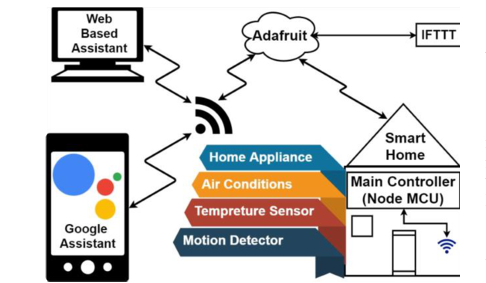
\includegraphics[width=1\textwidth]{Image/Fig. 1 Structure.png}
		\caption{\centering \textbf{Kiến trúc hệ thống tự động hóa nhà thông minh}}
		%\label{fig:QR-Code}
	\end{figure}

\end{frame}

% Slide 12
\begin{frame}[c]{\nameref{section4}}
	\textbf{Yêu cầu hệ thống}

	\vspace{1em}
	
	\begin{itemize}
		
		\setlength\itemsep{1.5em}

		\item{\textit{NodeMCU}: Nền tảng mã nguồn mở}
		
		\item{\textit{IFTTT(If This Then That)}: Dịch vụ trung gian}
		
		\item{\textit{Adafruit}: Máy chủ server, nơi lưu trữ dữ liệu thiết bị }
		
		\item{\textit{Arduino IDE}: Phần mềm lập trình Arduino}

		\item{\textit{Sensor}: Các cảm biến}

	\end{itemize}
\end{frame}

% Slide 13

\begin{frame}[c]{\nameref{section4}}
		
		\begin{columns}
			\begin{column}{0.4\textwidth}

				\textbf{ESP8266 NodeMCU}

				\vspace{1em}

				ESP8266 là một mạch vi điều khiển có thể giúp chúng ta điều khiển các thiết bị điện tử. 
		
				\vspace{2em}

				Điều đặc biệt của nó, đó là sự kết hợp của module Wifi tích hợp sẵn bên trong con vi điều khiển chính.

			\end{column}

			\begin{column}{0.6\textwidth} 
				\begin{figure}[h]
					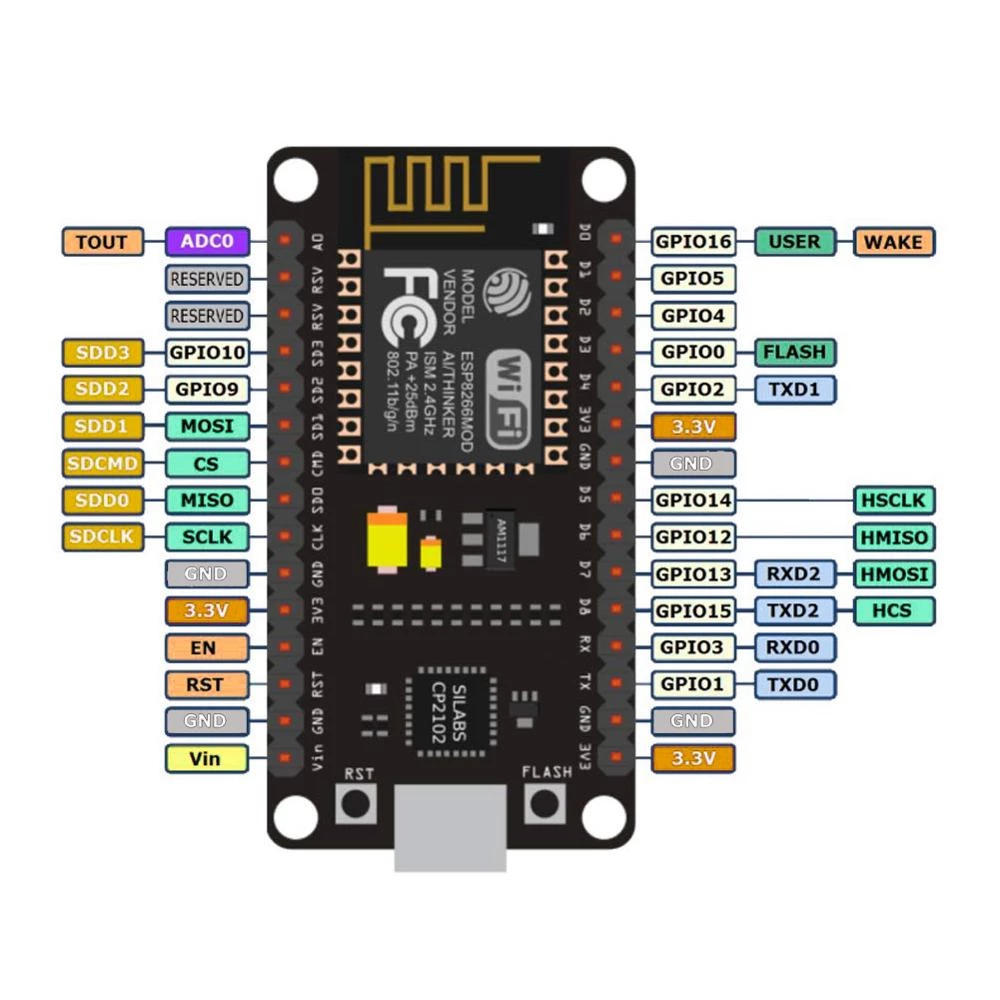
\includegraphics[width=1\textwidth]{Image/Fig. 2 ESP8266.jpg}
					\caption{\centering \textbf{Module ESP8266 NodeMCU}}
					%\label{fig:QR-Code}
				\end{figure}			
			\end{column}
		\end{columns}

\end{frame}

% Slide 14

\begin{frame}[c]{\nameref{section4}}
		
	\begin{columns}
		\begin{column}{0.55\textwidth}

			\textbf{Nguyên lý hoạt động}

			\vspace{1em}

			Bước 1: Kiểm tra kết nối Internet

			\vspace{0.5em}

			Bước 2: Kết nối ứng dụng tới điện thoại/Web của người dùng

			\vspace{0.5em}

			Bước 3: Xác minh người dùng bằng tài khoản/mã code/mật khẩu

			\vspace{0.5em}

			Bước 4: Người dùng ra lệnh điều khiển hệ thống

			\vspace{0.5em}

			Bước 5: Hệ thống BẬT/TẮT thiết bị theo yêu cầu
			

		\end{column}

		\begin{column}{0.45\textwidth} 
			\begin{figure}[h]
				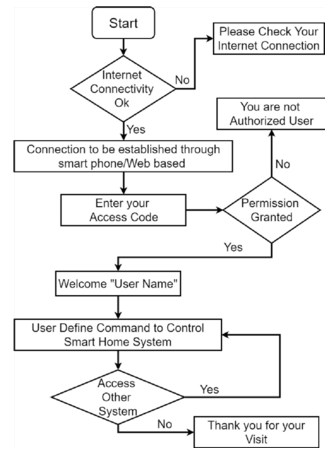
\includegraphics[width=1\textwidth]{Image/Fig. 3 Diagram.png}
				\caption{\centering \textbf{Sơ đồ nguyên lý}}
				%\label{fig:QR-Code}
			\end{figure}			
		\end{column}
	\end{columns}
	
\end{frame}

% Slide 15

\begin{frame}[c]{\nameref{section4}}
		
	\begin{figure}[h]
		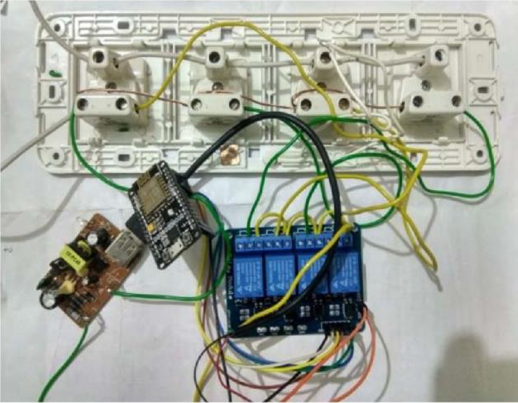
\includegraphics[width=0.8\textwidth]{Image/Fig. 4 Circuit.png}
		\caption{\centering \textbf{Lắp ráp mạch thật}}
		%\label{fig:QR-Code}
	\end{figure}			
	
\end{frame}

% Slide 16

\begin{frame}[c]{\nameref{section4}}
		
	\begin{figure}[h]
		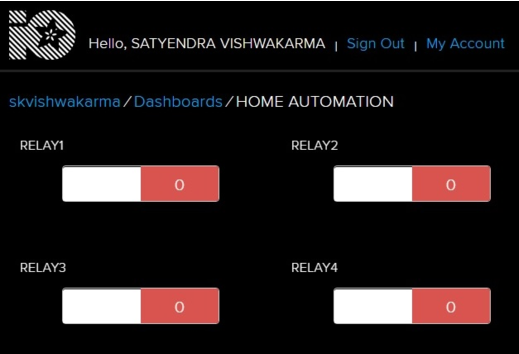
\includegraphics[width=0.9\textwidth]{Image/Fig. 5 Adafruit UI.png}
		\caption{\centering \textbf{Giao diện trên Adafruit}}
		%\label{fig:QR-Code}
	\end{figure}			
	
\end{frame}

% Slide 17

\begin{frame}[c]{\nameref{section4}}
		
	\begin{figure}[h]
		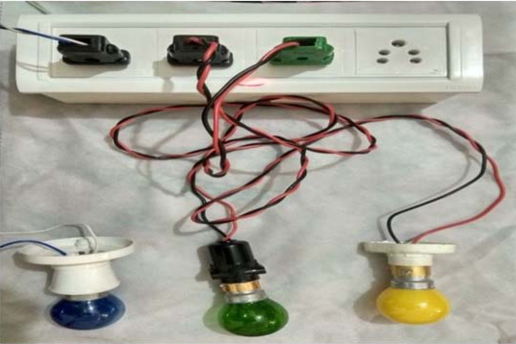
\includegraphics[width=0.9\textwidth]{Image/Fig. 6 Items.png}
		\caption{\centering \textbf{Các thiết bị được điều khiển}}
		%\label{fig:QR-Code}
	\end{figure}			
	
\end{frame}

% Slide 18

\begin{frame}[c]{\nameref{section4}}
		
	\textbf{Bảo mật hệ thống}

	\vspace{2em}

	Google Assistant sử dụng để điều khiển/giám sát ngôi nhà và trong trường hợp chạy nền(Background), hệ thống tự động hoá có thể kết nối thông qua dịch vụ trên web

	\vspace{1em}

	Để đảm bảo tính bảo mật, ứng dụng sẽ cung cấp mã truy cập, Google Assistant sẽ yêu cầu mã xác minh để tránh truy cập trái phép
	
\end{frame}

% Slide 19

\section{5 Kết luận}
\label{section5}

% Slide 20

\begin{frame}[c]{\nameref{section5}}

	Với sự trợ giúp của bộ điều khiển thiết kế, thiết bị gia dụng có thể được chuyển đổi thành một thiết bị thông minh và thông minh bằng việc sử dụng nhúng IoT
	
	\vspace{2em}
	
	Hoạt động của mô hình đề xuất đã được thể hiện bằng thực nghiệm với sự trợ giúp của việc kết nối ba bóng đèn

\end{frame}

% Slide 21

\begin{frame}[c]{\nameref{section5}}

	\textbf{Ưu điểm}

	\vspace{1em}

	\begin{itemize}

		\setlength\itemsep{1em}

		\item{Có thể giám sát và truy cập ngôi nhà thông minh của mình một cách dễ dàng từ mọi nơi}
		
		\item{Có tác dụng giúp đỡ người già và người khuyết tật}

	\end{itemize}

	\vspace{1em}

	\textbf{Hạn chế}

	\vspace{1em}

	\begin{itemize}

		\setlength\itemsep{1em}

		\item{Chưa chứng minh được sự ổn định nếu quy mô lớn có nhiều thiết bị}
		
	\end{itemize}

\end{frame}


% Slide 22
\begin{frame}[standout]
	\flushleft
	\Huge
	Thanks for watching!
\end{frame}

	
\end{document}
